%%
%% This is file `sample-acmlarge.tex',
%% generated with the docstrip utility.
%%
%% The original source files were:
%%
%% samples.dtx  (with options: `acmlarge')
%% 
%% IMPORTANT NOTICE:
%% 
%% For the copyright see the source file.
%% 
%% Any modified versions of this file must be renamed
%% with new filenames distinct from sample-acmlarge.tex.
%% 
%% For distribution of the original source see the terms
%% for copying and modification in the file samples.dtx.
%% 
%% This generated file may be distributed as long as the
%% original source files, as listed above, are part of the
%% same distribution. (The sources need not necessarily be
%% in the same archive or directory.)
%%
%%
%% Commands for TeXCount
%TC:macro \cite [option:text,text]
%TC:macro \citep [option:text,text]
%TC:macro \citet [option:text,text]
%TC:envir table 0 1
%TC:envir table* 0 1
%TC:envir tabular [ignore] word
%TC:envir displaymath 0 word
%TC:envir math 0 word
%TC:envir comment 0 0
%%
%%
%% The first command in ythe LaTeX source must be the \documentclass command.
\documentclass[acmlarge]{acmart}

%%ss[STYLE]{acmart}
%% \BibTeX command to typeset BibTeX logo in the docs
\AtBeginDocument{%
  \providecommand\BibTeX{{%
    \normalfont B\kern-0.5em{\scshape i\kern-0.25em b}\kern-0.8em\TeX}}}

%% Rights management information.  This information is sent to you
%% when you complete the rights form.  These commands have SAMPLE
%% values in them; it is ythe responsibility as an author to replace
%% the commands and values with those provided to you when you
%% complete the rights form.
\setcopyright{acmcopyright}
\copyrightyear{2022}
\acmYear{2022}
\acmDOI{}


%%
%% These commands are for a JOURNAL article.
\acmJournal{POMACS}
\acmVolume{37}
\acmNumber{4}
\acmArticle{3}
\acmMonth{8}

%%
%% Submission ID.
%% Use this when submitting an article to a sponsored event. You'll
%% receive a unique submission ID from the organizers
%% of the event, and this ID should be used as the parameter to this command.
%%\acmSubmissionID{123-A56-BU3}

%%
%% The majority of ACM publications use numbered citations and
%% references.  The command \citestyle{authoryear} switches to the
%% "author year" style.
%%
%% If you are preparing content for an event
%% sponsored by ACM SIGGRAPH, you must use the "author year" style of
%% citations and references.
%% Uncommenting
%% the next command will enable that style.
%%\citestyle{acmauthoryear}

%%
%% end of the preamble, start of the body of the document source.
\begin{document}

%%
%% The "title" command has an optional parameter,
%% allowing the author to define a "short title" to be used in page headers.
\title{Paper Reading of \textit{Pastry: Scalable, distributed object location and routing for large-scale peer-to-peer systems}}

%%
%% The "author" command and its associated commands are used to define
%% the authors and their affiliations.
%% Of note is the shared affiliation of the first two authors, and the
%% "authornote" and "authornotemark" commands
%% used to denote shared contribution to the research.
\author{Yiwei Yang}
\email{yangyw@shanghaitech.edu.cn}
\orcid{0000-0001-8011-5868}
\affiliation{
  \institution{ShanghaiTech University}
  \streetaddress{1 R.D. Zhongke}
  \city{Shanghai}
  \state{Shanghai}
  \country{China}
  \postcode{21210}
}

%%
%% By default, the full list of authors will be used in the page
%% headers. Often, this list is too long, and will overlap
%% other information printed in the page headers. This command allows
%% the author to define a more concise list
%% of authors' names for this purpose.
\renewcommand{\shortauthors}{Yiwei Yang}

%%
%% The abstract is a short summary of the work to be presented in the
%% article.
\begin{abstract}
  Peer-to-peer systems have previously gained popularity as a result of applications that have been created on top of them, such as file sharing apps. They're also fascinating in terms of research because they might be used to create a variety of network applications. Pastry and Chord are two protocols used to build peer-to-peer systems, and this study compares and contrasts their performance. They are classified as a peer-to-peer system of the second generation. The benefits and drawbacks of Pastry DHT will be discussed in this paper reading.
\end{abstract}

%%
%% The code below is generated by the tool at http://dl.acm.org/ccs.cfm.
%% Please copy and paste the code instead of the example below.
%%
\begin{CCSXML}
  <ccs2012>
  <concept>
  <concept_id>10010520.10010553.10010562</concept_id>
  <concept_desc>Distributed Systems~P2P System</concept_desc>
  <concept_significance>500</concept_significance>
  </concept>
  </ccs2012>
\end{CCSXML}

\ccsdesc[500]{Distributed System~Scalable System}
\ccsdesc[300]{Peer-to-peer system}


%%
%% Keywords. The author(s) should pick words that accurately describe
%% the work being presented. Separate the keywords with commas.
\keywords{}


%%
%% This command processes the author and affiliation and title
%% information and builds the first part of the formatted document.
\maketitle

\section{Strong point of the document}

\subsection{The paper introduced a Decentralized Hash Table}
For Single node, we have hash table to store the key value, when we scale the key value store into distributed system, we are able to have following properties:
\begin{figure}[htbp]
  \centering
  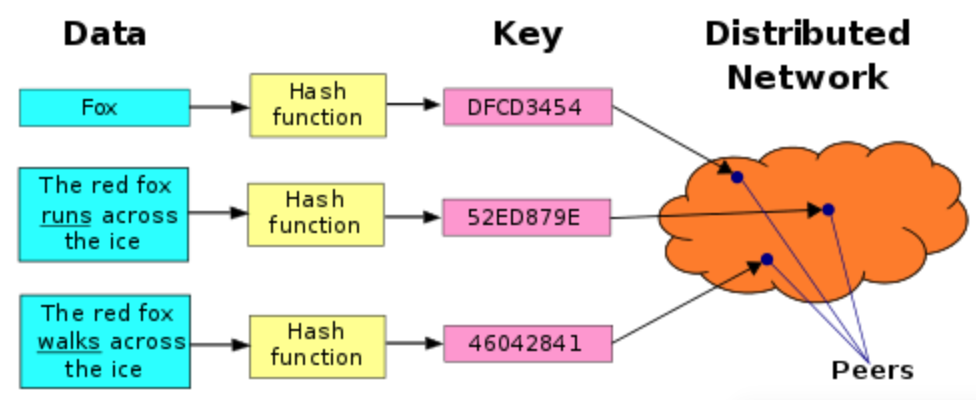
\includegraphics[width=0.6\columnwidth]{./distributed.png}
  \caption{From single node to distributed p2p system\cite{wikipedia}]}
\end{figure}
\begin{itemize}
  \item Autonomy and decentralization: The system is formed by the nodes collectively, without any central coordination.
  \item Fault Tolerance: Even if nodes are constantly joining, departing, and failing, the system should be dependable (in some sense).
  \item Scalability: the system should be able to handle thousands or millions of nodes with ease.
\end{itemize}
\begin{figure}[htbp]
  \centering
  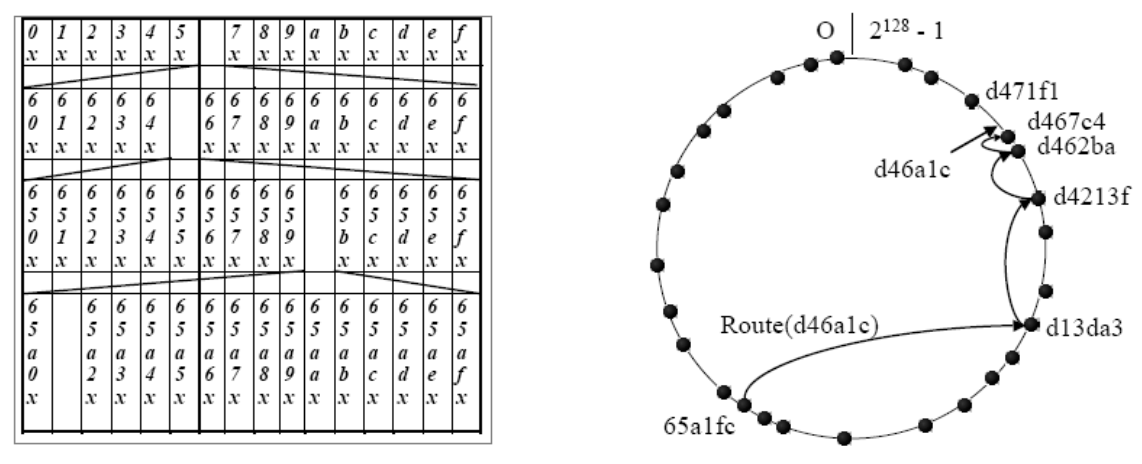
\includegraphics[width=0.6\columnwidth]{./genral.png}
  \caption{An example of Pastry DHT \cite{radkepastry}}
\end{figure}
\subsubsection{The Metrics are easy to record and store}
\begin{enumerate}
  \item Node and Message IDs

        IDs are simply 128 bits that can be used to uniquely identify a message or node. Note that node and message IDs are in the same format. They can be visualised as a single circle, like a clock; at the top of the circle is 0, and it counts up until it gets to $2^{128}-1$ (which is the maximum possible value an ID can hold), which sets next to 0. Thus the number line loops around, ensuring that there is always an ID which is modularly greater than the current ID and an ID that is modularly less than the current ID.

        IDs are the only metric used when actually routing a Message, as will be explained.

  \item Proximity

        Each node in the cluster keeps a "proximity metric" for every other node it knows about in the cluster. The proximity metric is simply a measurement of how close in the network topology one node is to another. Currently, this is measured by the time a single request takes between two nodes, and is updated every time the nodes communicate. For performance reasons, there is also a basic cache of proximity scores for nodes (both known and unknown) that the current node has encountered. This cache empties itself every hour, but is unbounded in the memory it can consume.

        Proximity is only used when populating state tables. The proximity is never used during routing itself.
\end{enumerate}
\subsubsection{The State Tables have bounded entry}

Pastry maintains three state tables, arrays of known nodes in the cluster that are used either for routing or maintaining the other state tables.
\begin{enumerate}
  \begin{figure}[htbp]
    \centering
    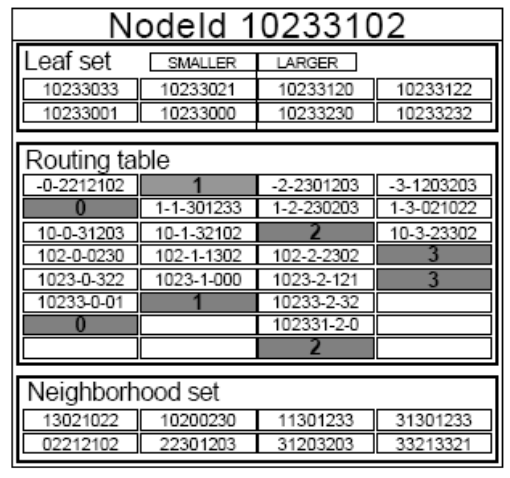
\includegraphics[width=0.6\columnwidth]{./neighbor_set.png}
    \caption{Example of State Tables}
  \end{figure}
  \item Routing Table
        On each side, the routing table is a two-dimensional array with 32 rows and 16 columns. In each column, a single node can be stored. For message routing, the routing table is utilized to store a representative fraction of the cluster.

        The routing table is filled by separating a node's ID into 32 digits, each of which has 16 possible possibilities. The common prefix between the current node and the node being inserted is used to determine which row a node belongs in.

        The routing table contains NodeIDs and their underlying physical network addresses with a prefix equal to the nodeID of the node containing these tables, with $\left|\log _{2^{b}} N\right|$ rows and $2^{\mathrm{b}}-1$ entries in each row.
  \item Leaf Set
        The leaf set can be represented as two 16-node arrays. The leaf set is used to keep track of the current node's immediate neighbors in the node ID space for routing purposes. The "left" array (of 16 nodes) contains nodes with lower IDs than the current node's ID. The other array (the "right") contains nodes with higher IDs than the present node.
  \item Neighborhood Set
        The neighborhood set is only a 32-node array. It exists to keep a list of the nodes in the network topology that are nearest to the current node, ensuring that the collection of known nodes has a diverse set of IDs. When populating and restoring the routing table, the neighborhood set is used, but not during routing.
\end{enumerate}
\subsubsection{routing within time complexity}
Routing a message through the cluster is a simple process of finding a suitable node in the state tables, then forwarding to that node. Should no suitable node be found, the message has reached its destination and is considered "delivered".

The message ID is the key tool used in routing the message through the cluster. The node with the ID closest to the message ID is the destination for the message, and each routing step should bring the message closer to that destination.

The first state table consulted when routing a message is the leaf set. If the message ID falls within the leaf set, then the current node knows the destination of the message, and forwards the message there.
\subsubsection{The soundness of joining the cluster without losing the information}
When a node wants to join the cluster, it has to know the IP address and port of another node. This node is assumed to be the one in the network topology closest to the joining node, albeit if a sub-optimal node is picked, only the routing locality properties will be altered. Pastry will be a little slower in general, but everything should still work.

The connecting node creates a message with the same node ID as it. This unique "join" message is then delivered to the selected node, which routes it normally. The routing table of each node that receives the message is sent to the joining node. Because it is presumed that the message was sent to the nearest node in the network topology, the sending node transmits its neighborhood set to the joining node, as nodes close to it should be close to the joining node. Finally, the message's destination node includes sending its leaf set to the joining node.

\section{Weak point of the document}
\subsection{The main concern of the decentralized system may be performance}
Pastry and Chord are peer-to-peer overlay networks that are self-organizing, robust, and effective. Pastry and Chord, as previously indicated, have theoretical lookup times of $\mathrm{O}(\log \mathrm{N})$, and node joins likewise take $\mathrm{O}(\log \mathrm{N})$ time. This time is obviously more than single node hash table which is nearly $\mathrm{O}(1)$.
\subsection{The decentralized algorithm is not secure and reliable}
\begin{figure}[htbp]
  \centering
  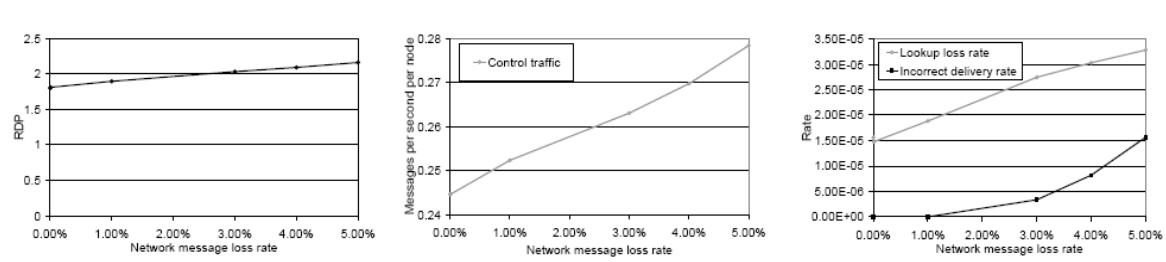
\includegraphics[width=0.6\columnwidth]{./network_packet_loss.png}
  \caption{Impact of Network packet loss rate on Pastry\cite{chandy1985distributed}}
\end{figure}
For example, the Packet loss between nodes will definitely result in data loss, we have to maintain the replica for the failure tolerance. RDP is the relative delay penalty ratio between delay achieved by Pastry and the network delay between these to nodes. The control traffic shows the control messages per node per second and the 3rd diagram in figure 8 shows the lookup loss rate and routing inconsistencies measured in the rate of incorrect routed messages. The stated data of these 3 diagrams show that Pastry scales very well with an increasing rate of packet loss. Just the graph of routing inconsistencies seems to grow more then strait proportional.
\section{Possible Refinement to the idea}
\subsection{Filesystem showcase \cite{rowstron2001storage}}
The pure key value store is not sufficient for production use. PAST is a distributed file system built on top of Pastry. The hash of a filename is computed before it is stored in the system. The contents of the file are then sent to the node in the circular keyspace that is closest to the hash computed from the filename. The file will then be sent to the k nodes closest to the actual key, the majority of which are likely to be leaf nodes of this node and so directly reachable. Data is retrieved by rehashing the file name and forwarding a data request across Pastry to the correct location in the keyspace. Any of the k nodes that have copies of the data can fulfill the request. This ensures data redundancy as well as load distribution.

\subsection{Cast more experiment to reduce the time bound of fault tolerance to make the system more stable}
The stabilizing techniques presented in the cited papers\cite{azmy2018machine}, Pastry's and Chord's, theoretically scale like the join and lookup in  $\mathrm{O}(\log \mathrm{N})$. The experimental findings appear to back up this theoretical top limit.
\bibliographystyle{ACM-Reference-Format}
\bibliography{pastry_scalable_distributed_object_location_and_routing_for_large_scale_peer_to_peer_systems}

\end{document}
\endinput
%%
%% End of file `sample-acmlarge.tex'.
